\documentclass{beamer}

\usepackage{graphicx,float,caption}
\usepackage{subcaption}
\usepackage{mdframed}
\usepackage{xcolor}
\usepackage{lipsum}
\usepackage{multimedia}
\usepackage{amsmath}
\usepackage[english]{babel}

\setbeamertemplate{footline}[frame number]

\usetheme{Warsaw}

\defbeamertemplate*{footline}{shadow theme}
{%
\leavevmode%
  \hbox{\begin{beamercolorbox}[wd=.5\paperwidth,ht=2.5ex,dp=1.125ex,leftskip=.3cm plus1fil,rightskip=.3cm]{author in head/foot}%
    \usebeamerfont{author in head/foot}\insertframenumber\,/\,\inserttotalframenumber\hfill\insertshortauthor
  \end{beamercolorbox}%
  \begin{beamercolorbox}[wd=.5\paperwidth,ht=2.5ex,dp=1.125ex,leftskip=.3cm,rightskip=.3cm plus1fil]{title in head/foot}%
    \usebeamerfont{title in head/foot}\insertshorttitle%
  \end{beamercolorbox}}%
  \vskip0pt%
}
\setbeamertemplate{caption}[numbered]

\title { Bayesian Reinforcement Learning Methods }
\subtitle { Using Bayesian MDPs and GPTD Methods }

\author[Vickie Ye and Alexandr Wang]
{ Vickie~Ye and Alexandr~Wang}

\date[Spring 2016]
{ May 12, 2016}

\begin{document}

\begin{frame}
\titlepage
\end{frame}

\begin{frame}{Markov Decision Processes}

\begin{itemize}
\item System described by a known set of states $S$ and actions $A$,
and unknown reward function $R(s, a)$ and transition function
$T(s, a, s') = P(X^{(t+1)} = s' | X^{(t)} = s, Y^{(t)} = a)$.
\item We define a quality function
$$Q = \sum_{t=0}^\infty \gamma^t R^{(t)},$$
which we approximate for each state-action pair as
$$Q(s, a) = \mathbb{E}[R(s,a)]+\gamma\sum_{s'}T(s, a, s')
\textrm{max}_{a'} Q(s',a').$$
\item To estimate $Q$, we need to estimate $T$ and $R$.
\end{itemize}
\end{frame}

\begin{frame}{Estimating $T$ with a Bayesian model}
We model our observed transition counts for each $(s, a)$ as
\begin{align*}
\mathbf{m}^{(t)} &\sim \textrm{Mult}(\pi(s, a))\\
\pi(s, a) &\sim \textrm{Dirichlet}(\mathbf{\alpha})
\end{align*}
where 
\begin{equation*}
\mathbf{\pi}(s, a) = (T(s, a, s_0), ..., T(s, a, s_{N-1})),
\end{equation*}
Our posterior is then 
\begin{equation*}
\mathbf{\pi}^{(t)}| D \sim \textrm{Dirichlet}(\mathbf{\alpha}^{(t)}|
\mathbf{m}^{(t)}), \;
\alpha^{(t)}_i = \alpha_i + m_i^{(t)}
\end{equation*}
\end{frame}

\begin{frame}{Estimating $R$ with a Bayesian model}
We model our reward $R(s, a)$ for each state-action pair as
\begin{align*}
r(s, a) &\sim \mathcal{N}(\mu, \tau) \\
\mu &\sim \mathcal{N}(\mu_0, c_0\tau) \\
\tau &\sim \textrm{Ga}(\beta, \rho)
\end{align*}
Our posterior is then
$$\tau \sim \textrm{Ga}\Big(\beta + \frac{k}{2}, \rho + \frac{1}{2}\sum_i(r_i - \bar{r})^2
+ \frac{kc_0(\bar{r}-\mu_0)^2}{2(n+c_0)}\Big),$$
$$\mu \sim \mathcal{N}\Big(\frac{k\bar{r} + c_0\mu_0}{k + c_0}, (k+c_0)\tau\Big)$$
\end{frame}

\begin{frame}{Testing Problems}

\begin{figure}
\centering
\begin{minipage}{0.5\textwidth}
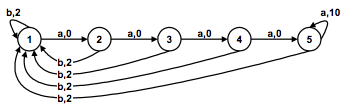
\includegraphics[width=\textwidth]{chain.png}
\caption{Chain Problem}
\end{minipage}%
\begin{minipage}{0.5\textwidth}
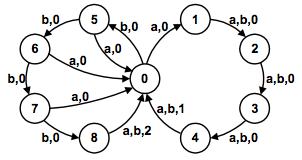
\includegraphics[width=\textwidth]{loop.png}
\caption{Loop Problem}
\end{minipage}%
\end{figure}

\begin{figure}
\begin{minipage}{0.3\textwidth}
\centering
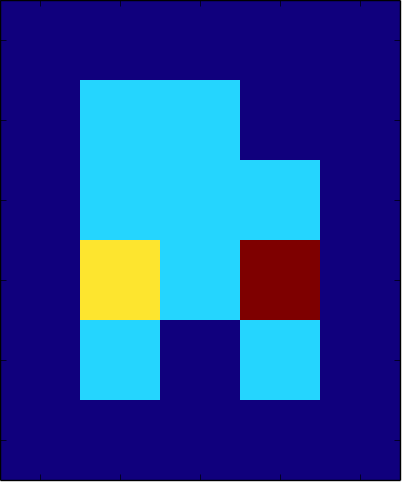
\includegraphics[width=0.8\textwidth]{easymaze.png}
\caption{Easy maze}
\end{minipage}%
\hspace{1cm}
\begin{minipage}{0.3\textwidth}
\centering
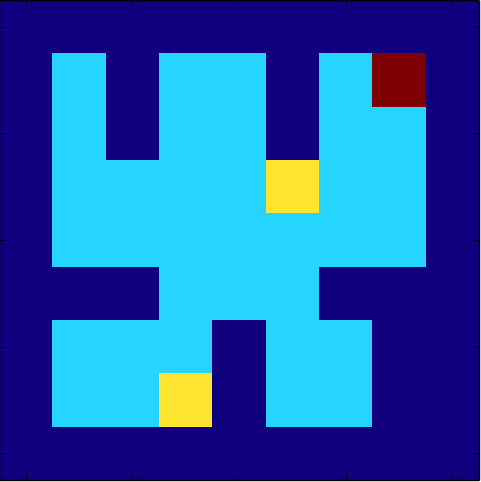
\includegraphics[width=\textwidth]{hardmaze.png}
\caption{Hard maze}
\end{minipage}%
\end{figure}
\end{frame}

\begin{frame}{Results on the Chain and Loop problems}
\begin{figure}
\centering
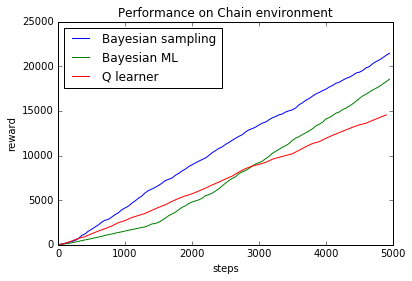
\includegraphics[width=0.5\textwidth]{chainPerf.png}
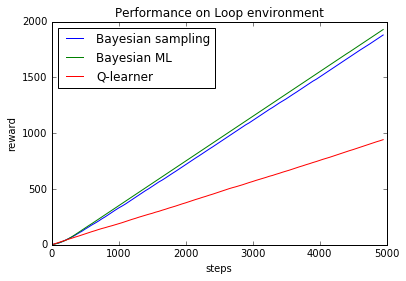
\includegraphics[width=0.5\textwidth]{loopPerf.png}
\end{figure}
\end{frame}

\begin{frame}{Results on the Maze problems}
\begin{figure}[!htb]
\centering
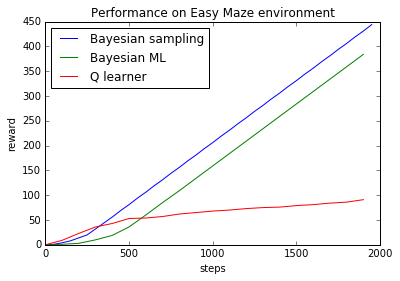
\includegraphics[width=0.5\textwidth]{smallMazePerf.png}
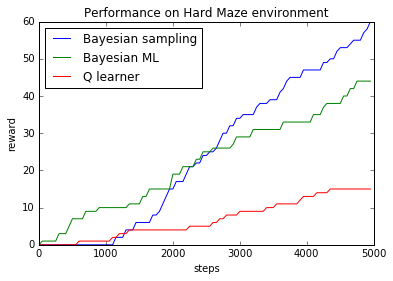
\includegraphics[width=0.5\textwidth]{largeMazePerf.png}
\end{figure}
\end{frame}

\end{document}
